% Created 2018-03-08 Thu 10:08
% Intended LaTeX compiler: pdflatex
\documentclass[11pt]{article}
\usepackage[letterpaper, margin=1.0in]{geometry}
\usepackage[utf8]{inputenc}
\usepackage[T1]{fontenc}
\usepackage{graphicx}
\usepackage{grffile}
\usepackage{longtable}
\usepackage{wrapfig}
\usepackage{rotating}
\usepackage[normalem]{ulem}
\usepackage{amsmath}
\usepackage{textcomp}
\usepackage{amssymb}
\usepackage{capt-of}
\usepackage{hyperref}

\author{Scott Trinkle}
\date{\today}
\title{Notes on (Spanne, 1988)}

\hypersetup{
 pdfauthor={Scott Trinkle},
 pdftitle={},
 pdfkeywords={},
 pdfsubject={},
 pdfcreator={Emacs 25.3.1 (Org mode 9.0.9)}, 
 pdflang={English}}

\begin{document}

\maketitle

\section{Brief overview of Spanne's derivation}
\label{sec:org400da3c}
Spanne assumes that \(N\), the number of detected photons is an uncorrelated 
Gaussian process. The variance of the estimate of \(\mu(x,y)\) is approximated by:

\begin{equation}
        \text{var}(\mu(x,y)) = \left(\frac{\pi}{m}\right)^2 \sum_{n_{\theta}=0}^m \sum_{n_R = -L/2}^{L/2} \frac{g^2(n_R\Delta R - R')}{E\{N(R',n_{\theta}\Delta\theta)\}}
\end{equation}

where: 
\begin{itemize}
\item \(m\) : number of views/angles
\item \(n_{\theta}\) : angular sampling index
\item \(n_R\) : sampling point index
\item \(g\) : filter function
\item \(E\{\}\) : denotes expectation
\item \(R'\) : radial coordinate
\item \(\Delta\theta\) : angular increment
\end{itemize}

Solving for the variance at an arbitrary pixel \((x,y)\) would involve finding all rays 
traversing that pixel, so Spanne simplifies things by looking at a single pixel in the 
center of a circular object, for which \(E\{N\}\) is equal for all angles. The variance then reduces to:


\begin{align}
  \text{var}(\mu(0,0)) &= \left(\frac{\pi}{m}\right)^2 \sum_{n_{\theta}=0}^m \sum_{n_R = -L/2}^{L/2} \frac{g^2(n_R\Delta R)}{E\{N(0,n_{\theta}\Delta\theta)\}} \nonumber \\
                       &= c_{filter} \left(\frac{\pi}{m}\right)^2 \sum_{n_{\theta}=0}^m \frac{1}{E\{N(0,n_{\theta}\Delta\theta)\}} \nonumber\\
                       &= c_{filter} \left(\frac{\pi^2}{m}\right) \frac{1}{E\{N(0,n_{\theta}\Delta\theta)\}} \label{eq:V}
\end{align}

where he has grouped the sum of squared filter terms into \(c_{filter}\) and exploited the fact that $E\{N(0,n_{\theta}\Delta\theta\}$ is
independent of $n_{\theta}$. Note also that the expectation for \(N\) is just the usual:

\begin{equation}
        E\{N(0,n_{\theta}\Delta\theta)\} = N_0 \text{exp}\left\{\sum_i \mu_i d_i\right\} \label{eq:E}
\end{equation}  

Spanne then defines the SNR as


\begin{equation}
        \frac{S}{\sigma} = \frac{|\mu_1 - \mu_2|}{\sqrt{\text{var}(\mu_1(0,0)) + \text{var}(\mu_2(0,0)}} \label{eq:snr}
\end{equation}


where \(\mu_1\) represents the attenuation in the central voxel \textit{without} any contrast material, and \(\mu_2\) 
represents the attenuation in the central voxel \textit{with} added contrast material. 

\section{Applications to our model}
\label{sec:orgf0bee3c}

Spanne includes a third material as a "shell" in his derivation. Ignoring that shell for our purposes, 
consider a homogeneous spherical object of diameter \(d\), with an attenuation coefficient \(\mu_1 \equiv \mu_{bg}\). Now, consider 
adding a small amount of contrast material to the central voxel, with voxel dimension \(r\) and attenuation 
coefficient \(\mu_c\), such that the total attenuation coefficient is now \(\mu_2 \equiv \mu_{bg} + \mu_c\). The SNR can then be calculated 
from equations \ref{eq:V}, \ref{eq:E} and \ref{eq:snr} to be:


\begin{equation}
        \left(\frac{S}{\sigma}\right)_{\text{Spanne}} = \sqrt{\frac{mN_0}{\pi^2 c_{filter}}}\frac{\mu_c}{\sqrt{\text{exp}\{\mu_{bg} d \} + \text{exp}\{\mu_c r + \mu_{bg} d }\}}
\end{equation}


Compare this to our working model: 

\begin{equation}
        \left(\frac{S}{\sigma}\right)_{\text{Ours}} = \sqrt{N_0} \mu_c \sqrt{\text{exp}\{-\mu_c  r - \mu_{bg} d\}}
\end{equation}

Besides the inclusion of energy-independent constants (including the reconstruction term, \(c_{filter}\)), the main 
difference is that our working model only incorporates the noise from the contrast-present case:

\begin{align}
  \sigma  &\propto \frac{1}{\bar{N}} \\
  \bar{N} &\equiv N_0 \text{exp}\{-\mu_c r - \mu_{bg} d\}
\end{align}  

whereas Spanne adds the variances from the contrast-present and contrast-absent cases in quadrature.

Comparisons of the two noise models (additional constants in Spanne model were not included) are shown below for a few values of contrast density. You can see that the Spanne model has generally the same shape,
but a lower overall value.

\begin{figure}[t]
  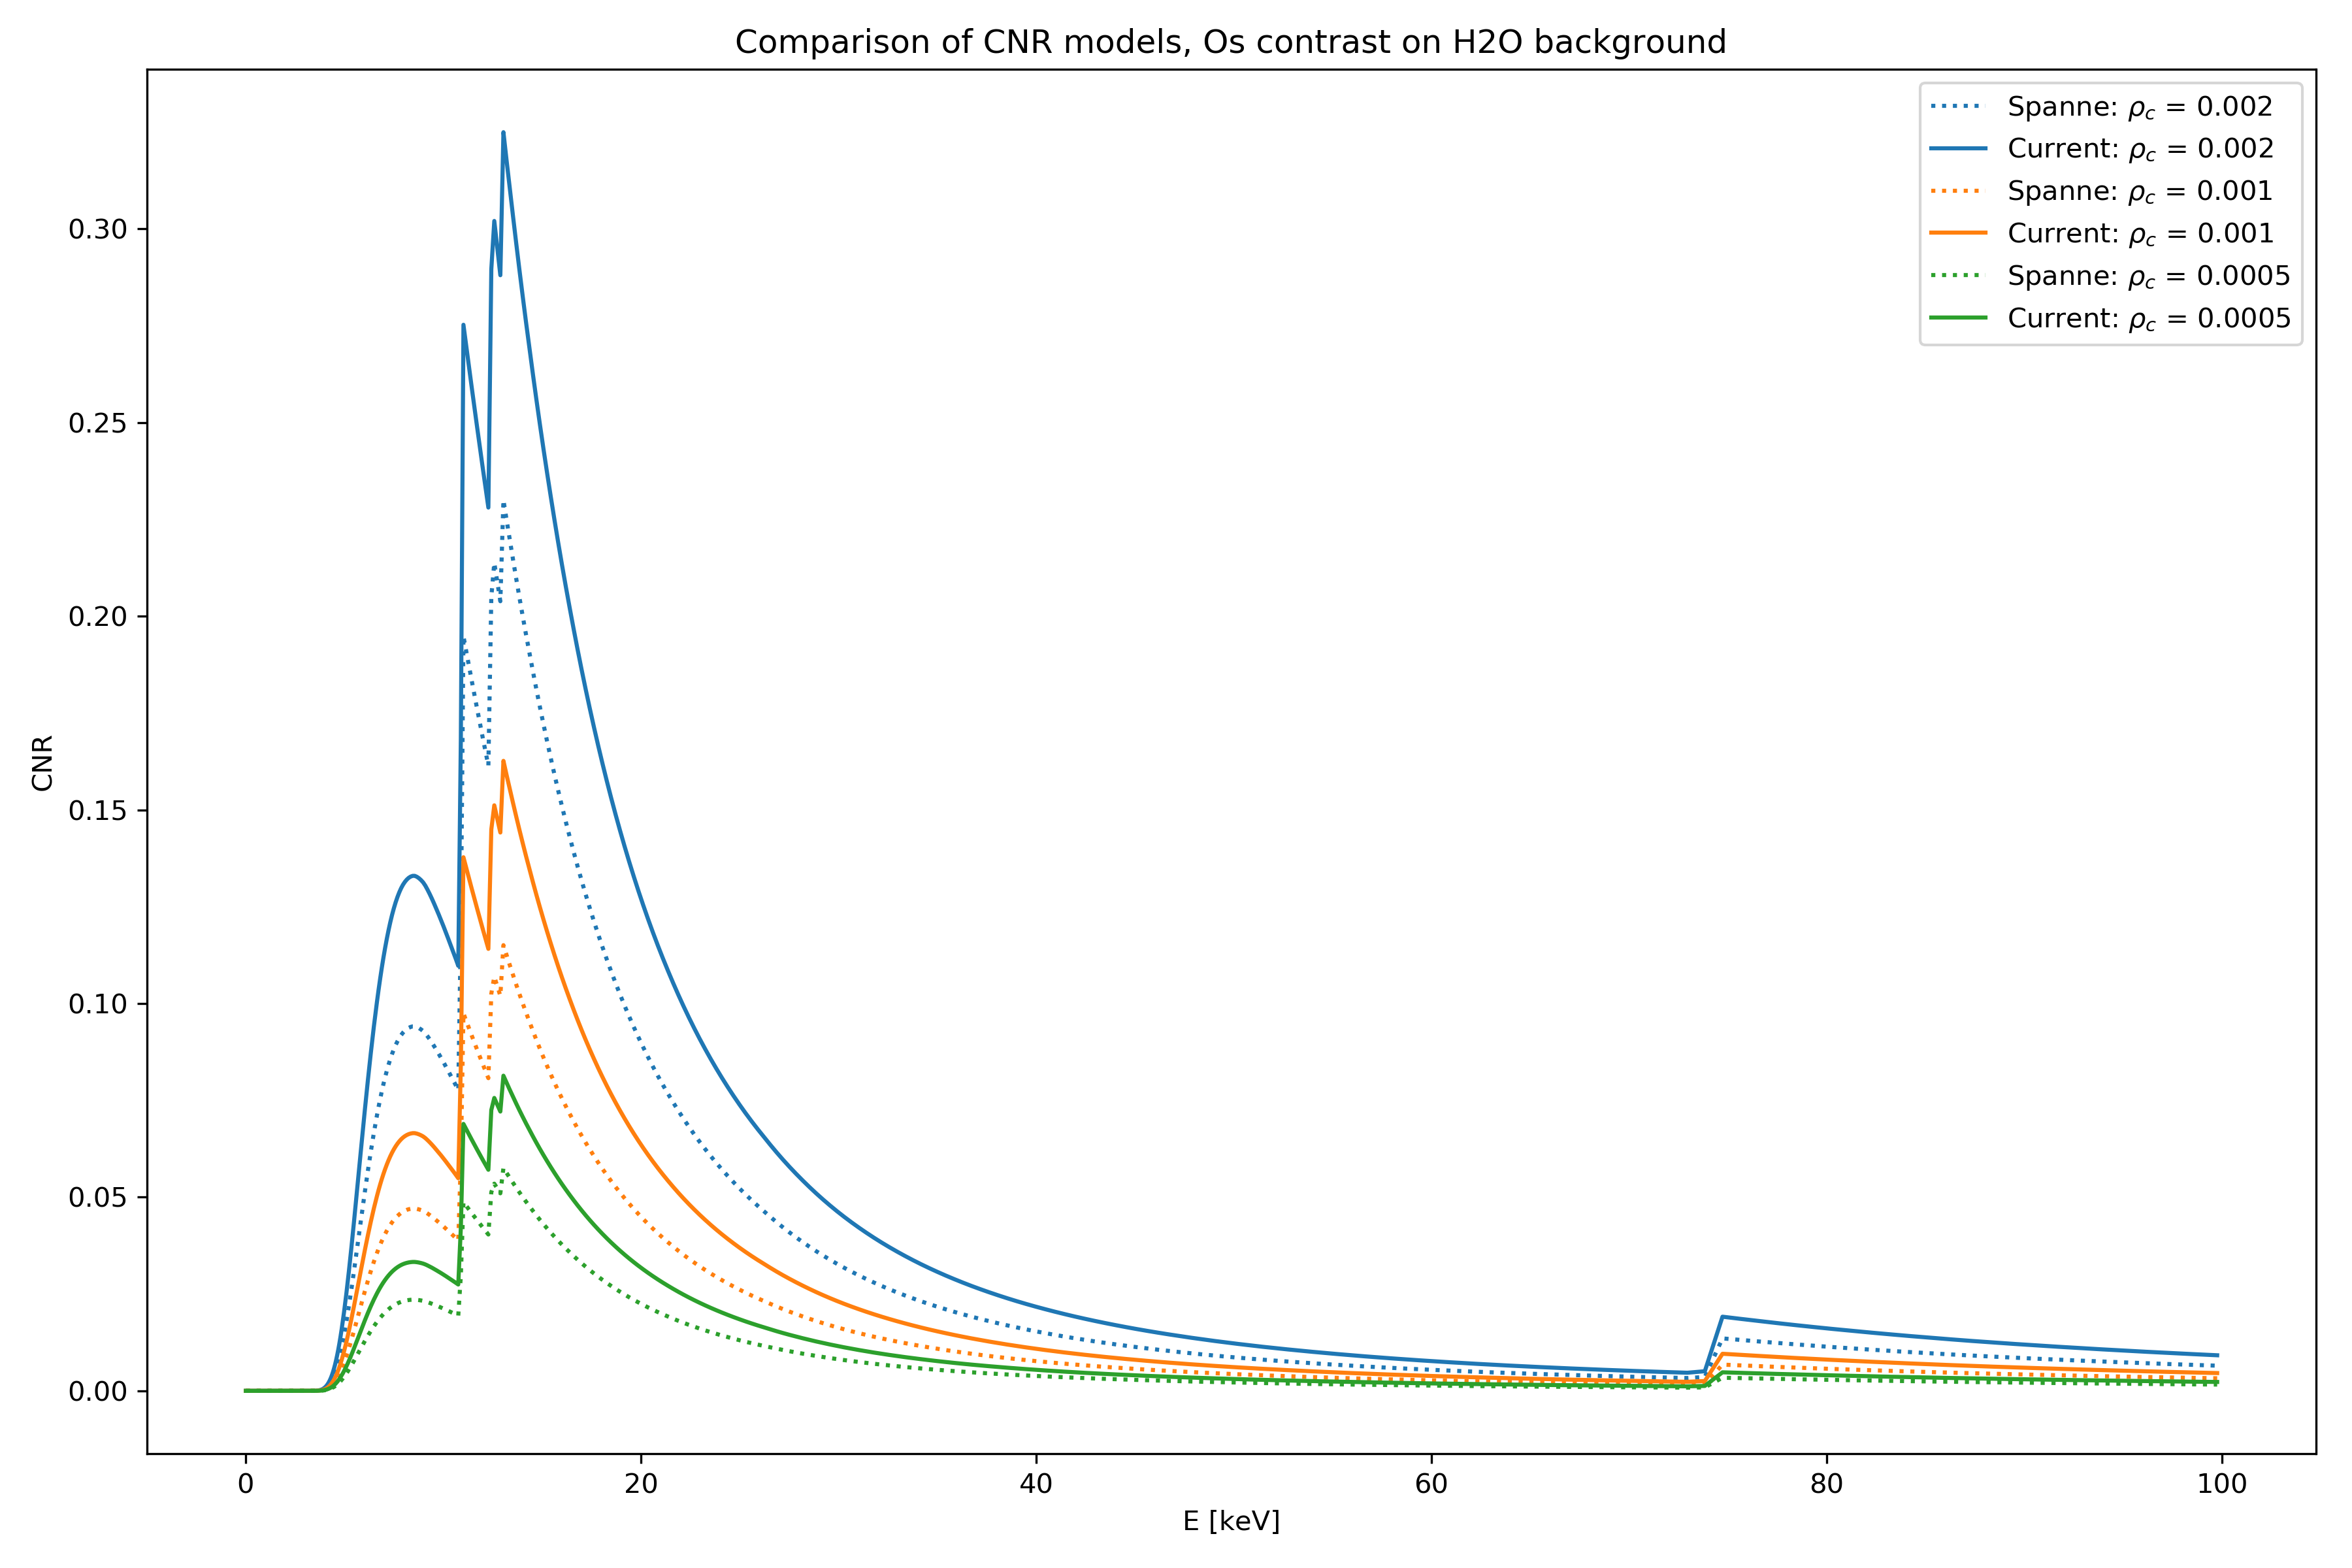
\includegraphics[width=\linewidth]{comparison}
\end{figure}


\end{document}

